\documentclass{beamer}

\usepackage{beamerthemesplit}
\usepackage{verbatim}
\usepackage[normalem]{ulem}

\usepackage{xcolor}

\definecolor{gold}{rgb}{1.,0.84,0.}
\definecolor{brightred}{rgb}{1.,0.4,0.4}
\definecolor{mygray}{RGB}{200,200,200}
\definecolor{lightsteelblue}{RGB}{176,196,222}
\definecolor{lightskyblue}{RGB}{135,206,250}
\definecolor{cadetblue}{RGB}{95,158,160}

\usetheme{default}
\usecolortheme{mule}

\usefonttheme{serif}

%\DeclareGraphicsExtensions{.pdf,.png,.jpg}

\newcommand{\snr}{$S/N$}
\newcommand{\snT}{$(S/N)_{\textrm{size}}$}
%\newcommand{\snT}{$\left( \frac{S}{N}\right)_{\textrm{size}}$}
\newcommand{\snflux}{$(S/N)_{\textrm{flux}}$}
%\newcommand{\snflux}{$\left( \frac{S}{N}\right)_{\textrm{flux}}$}

\newcommand{\lensfit}{\texttt{LENSFIT}}
\newcommand{\numba}{\texttt{Numba}}
\newcommand{\python}{\texttt{Python}}
\newcommand{\ngmix}{\texttt{ngmix}}
\newcommand{\shear}{{\bf g}}
\newcommand{\redmapper}{redMaPPer}
\newcommand{\est}{$e$}
\newcommand{\mest}{e}

\newcommand{\mcalR}{$R$}
\newcommand{\mcalRpsf}{$R^{p}$}
\newcommand{\mcalRS}{$R_{S}$}

\newcommand{\prelim}{{\bf{\it Preliminary}}}



\title{Overview of Multi-object Fitting}
\author{Erin Sheldon}
\institute{Brookhaven National Laboratory}

% http://texblog.net/latex-archive/plaintex/beamer-footline-frame-number/
% to add the page (frame ) number and not screw up the bottom line
% works for split themes?
\expandafter\def\expandafter\insertshorttitle\expandafter{%
      \insertshorttitle\hfill%
        \insertframenumber\,/\,\inserttotalframenumber}

% suppress navigation bar
\beamertemplatenavigationsymbolsempty
\setbeamertemplate{footline}{}

\begin{document}

\frame{\titlepage}


\setbeamertemplate{background canvas}[vertical shading][bottom=mgray,top=mblack]

\setbeamerfont*{itemize/enumerate body}{size=\Large}
\setbeamerfont*{itemize/enumerate subbody}{parent=itemize/enumerate body}
\setbeamerfont*{itemize/enumerate subsubbody}{parent=itemize/enumerate body}


\frame
{
    \frametitle{Multi-object Fitting: Motivation}

    \begin{itemize}

        \item Multi-band Multi-epoch Multi-object fitting

            \item Fitting for fluxes on coadd images is not ideal
        \begin{itemize}

            \item Chip boundaries result in discontinuities in image, including
                the effective PSF.

            \item Standard binary ``segmentation'' method for dealing with
                blending is sub-optimal; some light may still leak between
                neighbors.

        \end{itemize}
    \end{itemize}
}



\frame
{
    \frametitle{Multi-object Fitting (MOF)}

    \setbeamerfont*{itemize/enumerate body}{size=\large}
    \setbeamerfont*{itemize/enumerate subbody}{parent=itemize/enumerate body}
    \setbeamerfont*{itemize/enumerate subsubbody}{parent=itemize/enumerate body}
 
    \begin{itemize}

        \item Based on Erin Sheldon's {\color{gold} \ngmix} multi-band multi-epoch fitting
            \begin{itemize}

                \item Fit to all single-epoch images from all bands simultaneously
                \item Shape and radial profile common to all bands
                \item Different fluxes for each band {\color{gold} $g,r,i,z$}

            \end{itemize}

        \item Matt Becker added multi-{\color{gold}object} fitting
            \begin{itemize}
                \item Find groups of objects using a friends-of-friends algorithm
                \item Fit all objects simultaneously
                \item Accurately assign flux to objects:  Replaces binary
                    ``segmentation map'' approach.

            \end{itemize}


    \end{itemize}

\setbeamerfont*{itemize/enumerate body}{size=\Large}
\setbeamerfont*{itemize/enumerate subbody}{parent=itemize/enumerate body}
\setbeamerfont*{itemize/enumerate subsubbody}{parent=itemize/enumerate body}


}

{
    \setbeamertemplate{background canvas}[vertical shading][bottom=white,top=white]
    \frame
    {
        \frametitle{Example friends-of-friends group}

     
        \begin{center}
            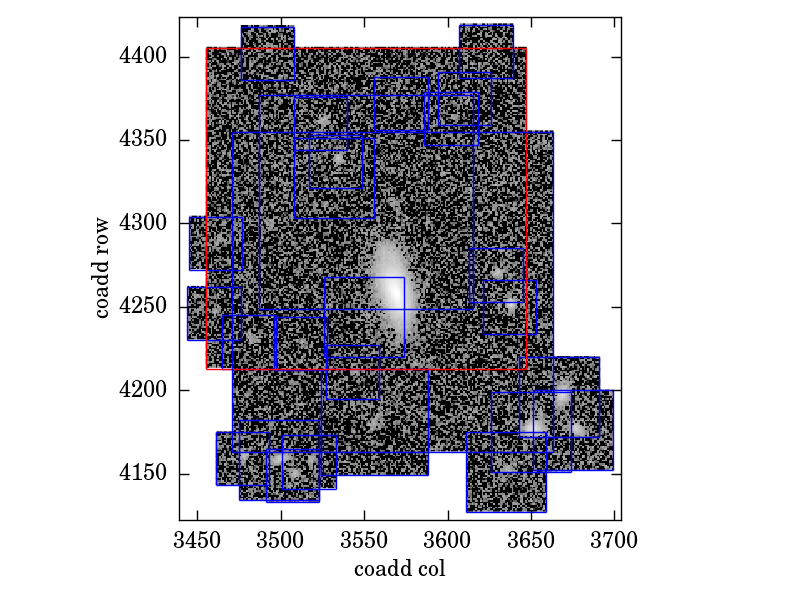
\includegraphics[width=\textwidth]{fof-001.png}
            \newline
        \end{center}


    }
    \setbeamertemplate{background canvas}[vertical shading][bottom=mgray,top=mblack]
}


\frame
{
    \frametitle{Multi-object Fitting (MOF)}

 
    \begin{itemize}

        \item Throwing it all into a single maximum likelihood fit would be unstable
            an expensive

        \begin{enumerate}
            \item Perform an initial fit to each object, masking neighbors

            \item Perform another fit, subtracting the light from neighbors based
                on previous fits

            \item Repeat 2 until all fits converge.
        \end{enumerate}

        \item Typically less than 15 iterations are required


    \end{itemize}

}


{
    \setbeamertemplate{background canvas}[vertical shading][bottom=white,top=white]
    \frame
    {
        \frametitle{Example Flux Splitting}

     
        \begin{center}
            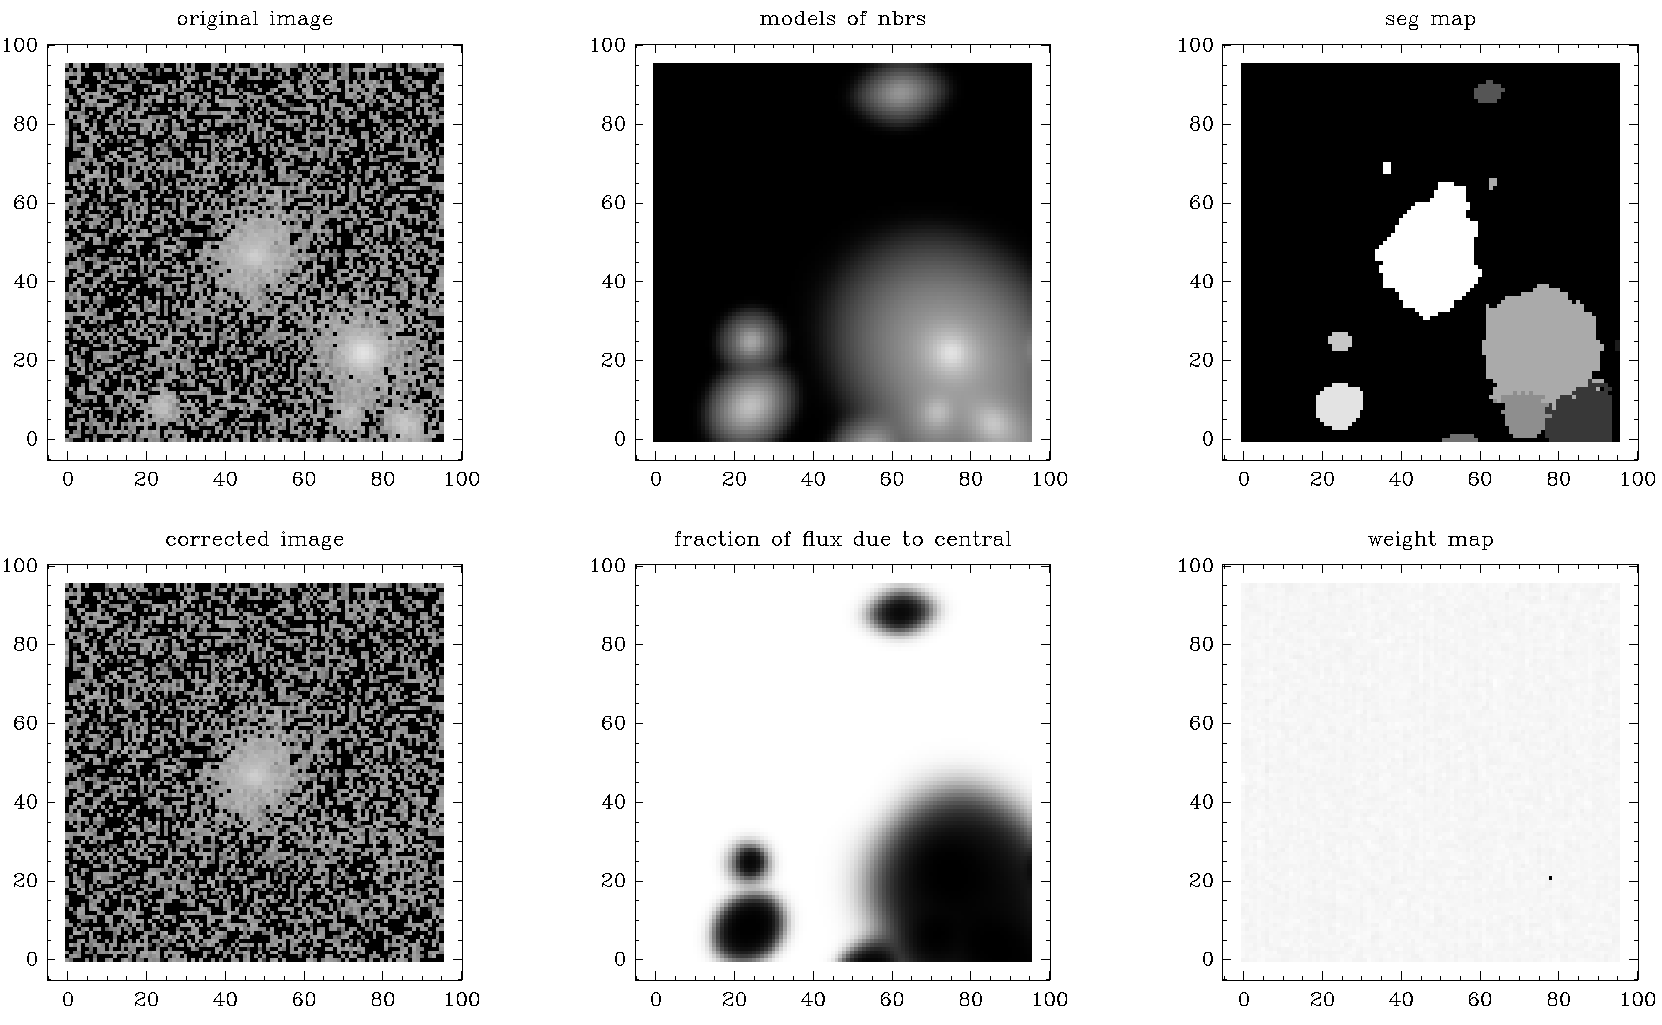
\includegraphics[width=\textwidth]{314469384-mb-cm-max-nbrs-band1-icut1-crop.png}
            \newline
        \end{center}


    }
    \setbeamertemplate{background canvas}[vertical shading][bottom=mgray,top=mblack]
}



\frame
{
    \frametitle{Performance}

    \begin{itemize}

        \item Improves photometry over coadd where there are image
            discontinuities.  E.g. where chip gaps are important.

        \item photozs:  $\sim$20\% improvement over mag-auto for clusters and individual
            galaxies

    \end{itemize}

}

\frame
{
    \frametitle{Extra Slides}


}




\frame
{
    \frametitle{Model}


    \begin{itemize}

        \item Modification of the SDSS composite model, aka the ``Sloan
            Swindle'' (Lupton).

        \item Constrained bulge+disk model.

            \begin{itemize}
                \item Informative priors on the center, bulge-fraction, and ellipticity
                \item Uninformative priors on the size and flux
            \end{itemize}


    \end{itemize}

}




\end{document}
